\section{Design}

%This is where the logical / abstract contribution of the project is presented.

%Notice that, when describing a software project, three dimensions need to be taken into account: structure, behaviour, and interaction.

%Always remember to report \textbf{why} a particular design has been chosen.
%Reporting wrong design choices which has been evalued during the design phase is welcome too.

In questa sezione esporremo il design del progetto, partendo dalle decisioni prese in ambito architetturale e proseguendo
col design di dettaglio.

\subsection{Design architetturale}
Come precedentemente illustrato nei capitoli precedenti, il progetto si propone di sviluppare un meccanismo per la creazione di sistemi multi-agente distribuiti utilizzando \textit{JaKTa}.
Il gruppo ha deciso di raggiungere questo obiettivo fornendo un'estensione del framework e del suo Domain Specific Language il più minimale possibile.
Dal punto di vista architetturale, il progetto si colloca come modulo a sé stante, come mostrato nella figura \ref{fig:architecture}:

\begin{figure}[ht]
    \centering
    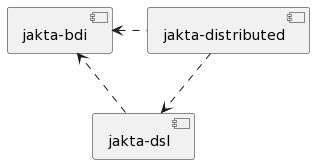
\includegraphics[width=0.8\textwidth]{figures/general-architecture.png}
    \caption{Architettura del progetto}
    \label{fig:architecture}
\end{figure}

In particolare, il modulo sviluppato è formato da tre componenti principali, come mostrato nella figura \ref{fig:detailed-architecture}:

\begin{figure}[ht]
    \centering
    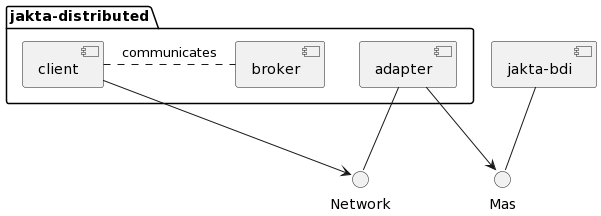
\includegraphics[width=0.8\textwidth]{figures/detailed-architecture.png}
    \caption{Architettura del modulo sviluppato}
    \label{fig:detailed-architecture}
\end{figure}

Come anticipato in precedenza, il progetto presenta anche un'estensione del Domain Specific Language di JaKTa, che permette di definire un sistema multi-agente con capacità di comunicare con l'esterno.

\begin{figure}[ht]
    \centering
    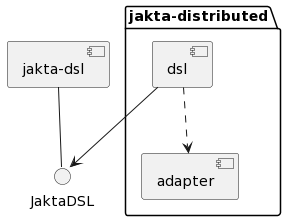
\includegraphics[width=0.8\textwidth]{figures/dsl-architecture.png}
    \caption{Architettura del Domain Specific Language}
    \label{fig:dmas-architecture}
\end{figure}

\begin{figure}
    \centering
    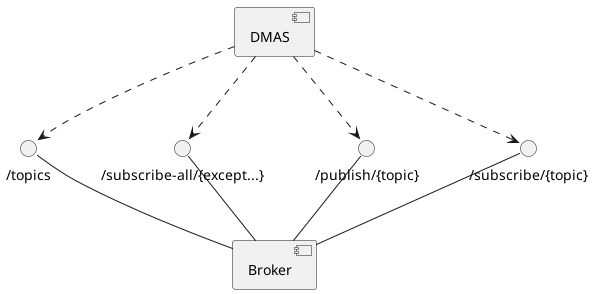
\includegraphics[width=0.8\textwidth]{figures/network-architecture.png}
    \caption{Architettura di rete}
    \label{fig:network-architecture}
\end{figure}

\subsection{Design di dettaglio}
La soluzione proposta consiste nell'implementazione di una versione alternativa dell'interfaccia \textit{Mas}, chiamata \textit{Dmas}, da utilizzare in contesti distribuiti.
Questa estensione dovrà comportarsi come un Mas, ma in aggiunta dovrà essere in grado di comunicare con altri Dmas attraverso la rete utilizzando un protocollo di comunicazione.

Come si può notare dalla figura \ref{fig:architecture}, il progetto è composto da tre componenti principali:

\subsubsection{Adapter}

\subsubsection{Client}

\begin{figure}
    \centering
    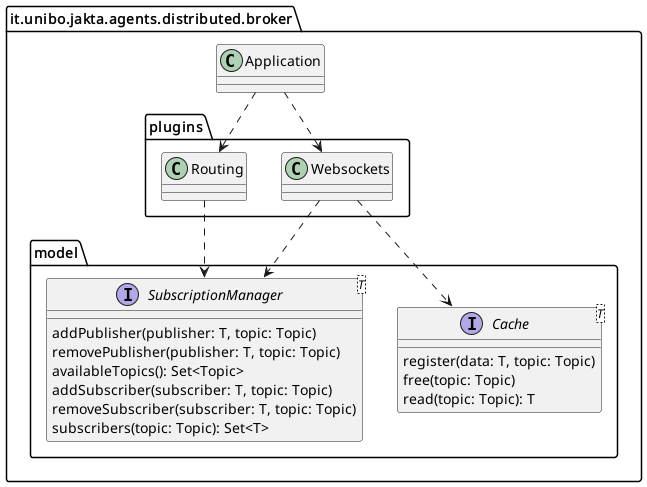
\includegraphics[width=0.8\textwidth]{figures/broker-class-diagram.png}
    \caption{Architettura di rete}
    \label{fig:broker-class-diagram}
\end{figure}

\subsubsection{Broker}


\subsection{Behaviour}

descrizione del main loop del DMas

\subsection{Interaction}

interazione tra vari DMas

interazione tra DMas, client e broker
